\documentclass{article}

\usepackage{graphicx}
\usepackage{tikz}
\usepackage{tikzsymbols}
\usetikzlibrary{calc,patterns,shapes.geometric}
\pagestyle{empty}
\usepackage[margin=0pt]{geometry}
\geometry{papersize={14in,12in}}

\def\centerarc[#1](#2)(#3:#4:#5){\draw[#1] ($(#2)+({#5*cos(#3)},{#5*sin(#3)})$) arc (#3:#4:#5);}

\begin{document}
	\begin{figure}
		\centering
		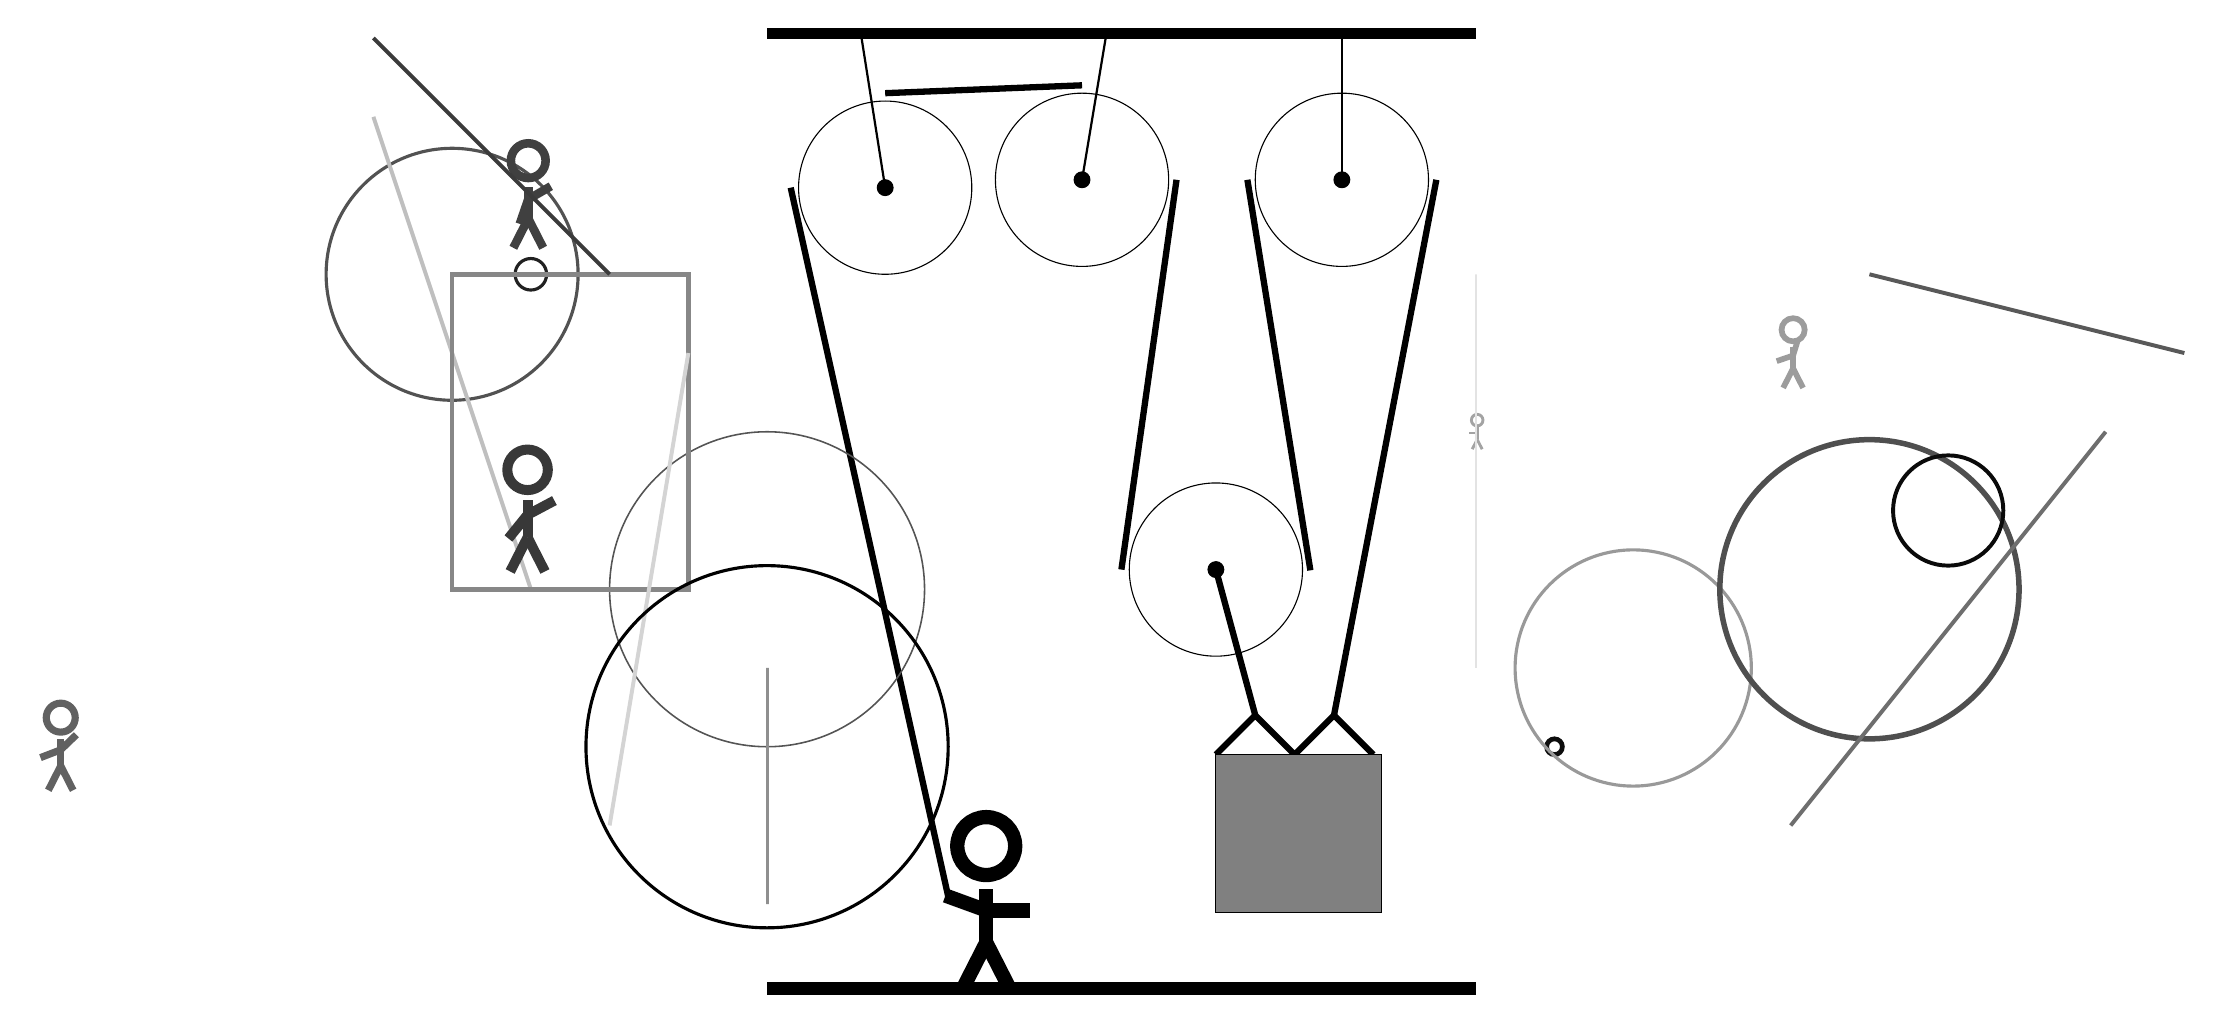
\begin{tikzpicture}
			%%%%% START %%%%%
			
			\draw[fill=black] (-3, 9) rectangle (6, 9.125);
			
			\draw (1, 7.2) circle (1.1);
			\draw[fill=black] (1, 7.2) circle (0.1);
			\draw[thick] (1, 7.2) -- (1.3, 9);
			
			\draw (4.3, 7.2) circle (1.1);
			\draw[fill=black] (4.3, 7.2) circle (0.1);
			\draw[thick] (4.3, 7.2) -- (4.3, 9);
			
			\draw (2.7, 2.25) circle (1.1);
			\draw[fill=black] (2.7, 2.25) circle (0.1);
			
			\draw[line width=0.8mm]  (2.7, -0.1) -- (3.2, 0.4) -- (3.7, -0.1) -- (4.2, 0.4) -- (4.7, -0.1);
			\draw[fill=black!50] (2.7, -0.1) rectangle (4.8, -2.1);
			
			\draw (-1.5, 7.1) circle (1.1);
			\draw[fill=black] (-1.5, 7.1) circle (0.1);
			\draw[thick] (-1.5, 7.1) -- (-1.8, 9);
			
			\draw[line width=0.8mm](-0.7, -1.9) --  (-2.7, 7.1);
			\centerarc[line width=0.8mm](-1.5, 7.1)(90:180:1.2000000000000002);
			\draw[line width=0.8mm](-1.5, 8.3) -- (1, 8.4);
			\centerarc[line width=0.8mm](1, 7.2)(0:90:1.2000000000000002);
			\draw[line width=0.8mm](2.2, 7.2) -- (1.5, 2.25);
			\centerarc[line width=0.8mm](2.7, 2.25)(180:370:1.2000000000000002);
			\draw[line width=0.8mm] (3.9, 2.24) -- (3.1, 7.2);
			\centerarc[line width=0.8mm](4.3, 7.2)(0:180:1.2000000000000002);
			\draw[line width=0.8mm](4.2, 0.4) -- (5.5, 7.2);
			\draw[line width=0.8mm] (3.2, 0.4) -- (2.7, 2.25);
			
			\node at (-0.2, -2) {\Strichmaxerl[10][-20][0]};
			
			\draw [line width=0.4mm, color=black!68](-7, 6) circle (1.6);
			
			\node[line width=0.2mm, color=black!75] at (-6, 7) {\Strichmaxerl[6][71][30]};
			\node[line width=0.2mm, color=black!36] at (6, 4) {\Strichmaxerl[2][0][87]};
			\draw [line width=0.4mm, color=black!87](-6, 6) circle (0.2);
			
			\draw[line width=0.2mm, color=black!11] (6, 1) rectangle (6, 6);
			\draw [line width=0.2mm, color=black!67](-3, 2) circle (2.0);
			\draw [line width=0.6mm, color=black!95](7, 0) circle (0.1);
			\draw[line width=0.5mm, color=black!65](11, 6) -- (15, 5);
			\draw[line width=0.5mm, color=black!25](-8, 8) -- (-6, 2);
			
			\node[line width=0.5mm, color=black!78] at (-6, 3) {\Strichmaxerl[7][51][28]};
			\draw[line width=0.6mm, color=black!47] (-4, 6) rectangle (-7, 2);
			
			\node[line width=0.6mm, color=black!39] at (10, 5) {\Strichmaxerl[4][19][73]};
			\draw[line width=0.4mm, color=black!44] (-3, -2) rectangle (-3, 1);
			\draw [line width=0.4mm, color=black!40](8, 1) circle (1.5);
			\draw [line width=0.7mm, color=black!69](11, 2) circle (1.9);
			\draw[line width=0.5mm, color=black!17](-4, 5) -- (-5, -1);
			\draw [line width=0.5mm, color=black!96](12, 3) circle (0.7);
			\draw[line width=0.5mm, color=black!77](-5, 6) -- (-8, 9);
			\node[line width=0.3mm, color=black!62] at (-12, 0) {\Strichmaxerl[5][21][44]};
			\draw[line width=0.5mm, color=black!57](10, -1) -- (14, 4);
			\draw [line width=0.4mm, color=black!100](-3, 0) circle (2.3);
			
			
			\draw[fill=black] (-3, -3) rectangle (6, -3.15);
			
			%%%%% END %%%%%
		\end{tikzpicture}
	\end{figure}	
\end{document}